\documentclass[12pt,letterpaper]{article}
\usepackage{fontspec}
\setmainfont{Arial}
\usepackage{setspace}
\usepackage[utf8]{inputenc}
\usepackage[portuguese]{babel}
\usepackage[version=3]{mhchem}
\usepackage[journal=jacs]{chemstyle}
\usepackage{listings}
\usepackage[affil-it]{authblk} 
\usepackage{tikz}
\usepackage{hyperref}
\usepackage{cite}
\usepackage{verbatim}
\usepackage{graphicx}
\usepackage{url}     
\usepackage{amsmath} 
\usepackage{tabularx}
\usepackage{ragged2e}
\usetikzlibrary{shapes.arrows}
\usepackage{siunitx}
\sisetup{mode=text, output-decimal-marker = {,}, per-mode = symbol, qualifier-mode = phrase, qualifier-phrase = { de }, list-units = brackets, range-units = brackets, range-phrase = --}
\DeclareSIUnit[number-unit-product = \;] \atmosphere{atm}
\DeclareSIUnit[number-unit-product = \;] \pound{lb}
\DeclareSIUnit[number-unit-product = \;] \inch{"}
\DeclareSIUnit[number-unit-product = \;] \foot{ft}
\DeclareSIUnit[number-unit-product = \;] \yard{yd}
\DeclareSIUnit[number-unit-product = \;] \mile{mi}
\DeclareSIUnit[number-unit-product = \;] \pint{pt}
\DeclareSIUnit[number-unit-product = \;] \quart{qt}
\DeclareSIUnit[number-unit-product = \;] \flounce{fl-oz}
\DeclareSIUnit[number-unit-product = \;] \ounce{oz}
\DeclareSIUnit[number-unit-product = \;] \degreeFahrenheit{\SIUnitSymbolDegree F}
\DeclareSIUnit[number-unit-product = \;] \degreeRankine{\SIUnitSymbolDegree R}
\DeclareSIUnit[number-unit-product = \;] \usgallon{galón}
\DeclareSIUnit[number-unit-product = \;] \uma{uma}
\DeclareSIUnit[number-unit-product = \;] \ppm{ppm}
\DeclareSIUnit[number-unit-product = \;] \eqg{eq-g}
\DeclareSIUnit[number-unit-product = \;] \normal{\eqg\per\liter\of{solución}}
\DeclareSIUnit[number-unit-product = \;] \molal{\mole\per\kilo\gram\of{solvente}}
\usepackage{cancel}
\usepackage{graphicx}
\usepackage{lmodern}
\usepackage{fancyhdr}
\usepackage[left=4cm,right=2cm,top=3cm,bottom=3cm]{geometry}
\usepackage{titlesec}
\usepackage{enumitem}
\titleformat*{\section}{\bfseries\large}
\titleformat*{\subsection}{\bfseries\normalsize}
\usepackage{float}
\floatstyle{plaintop}
\newfloat{anexo}{thp}{anx}
\floatname{anexo}{Anexo}
\restylefloat{anexo}
\restylefloat{figure}
\usepackage[margin=10pt,labelfont=bf]{caption}
\usepackage{todonotes}
\usepackage[affil-it]{authblk} 
\usepackage{babel}
\usepackage{tikz}
\usetikzlibrary{babel}
\usepackage{siunitx}

%======================================================================

\begin{document}
\onehalfspacing 
\thispagestyle{empty}

\begin{center}
\vspace{0.2cm}

\hrulefill

\textbf{UNIVERSIDADE FEDERAL DE ALAGOAS}\\
\textbf{PRÓ-REITORIA DE PESQUISA E PÓS-GRADUAÇÃO}\\
COORDENAÇÃO DE PESQUISA

\hrulefill

\vspace{0.5cm}

PROGRAMA INSTITUCIONAL DE BOLSAS DE INICIAÇÃO\\ CIENTÍFICA -- PIBIC CNPq/UFAL/FAPEAL

\vspace{1.0cm}

\textbf{\textit{\Large{RELATÓRIO FINAL \\ (2017 -- 2018)}}}\\

\vspace{1.2cm}

\textbf{TÍTULO DO PROJETO DE PESQUISA:}

\underline{Análise de Sinais e Imagens com Distâncias Estocásticas e Diferenças de Entropias}

\vspace{0.6cm}

\textbf{TÍTULO DO PLANO DE TRABALHO:}

\underline{Desenvolvimento de Bibliotecas para Simulação e Inferência em Modelos para Imagens SAR}

\end{center}

\textbf{\underline{NOME DO ORIENTADOR:}} Alejandro César Frery 

\vspace{0.4cm}

\textbf{\underline{NOME DO BOLSISTA:}} Marcos Gleysson Silva do Nascimento

\vspace{1cm}

\begin{table}[!h]
\begin{center}
\begin{tabularx}{\textwidth}{|X|X|X|X|}
\hline                              
\hspace{1.3cm} X & Bolsista CNPq &  &Bolsista FAPEAL\\
\hline             
& Bolsista UFAL &  &Colaborador\\
\hline     
\end{tabularx}
\end{center}
\end{table}

GRANDE ÁREA DO CONHECIMENTO (CNPq): Ciências  Exatas  e  da  Terra

SUB-ÁREA DO CONHECIMENTO (CNPq) : Matemática  da  Computação   

\vspace{0.5cm}

Projeto financiado:  \hspace*{1.5cm} Sim \hspace*{1.5cm} X Não

\vspace*{0.8cm}

\begin{center}

Maceió - AL, 15/08/2018

\end{center}

%=================================================================

\newpage
\section*{\centering \textbf{RESUMO}} % (Máximo 1 página – Sem parágrafos) 
%Tem no parcial

	A teoria da informação é um ramo da matemática que estuda quantificação da informação. Essa teoria teve seus pilares estabelecidos por Claude Shannon (1948) que formalizou conceitos com aplicações na teoria da comunicação e estatística. A teoria da informação foi desenvolvida originalmente para compressão de dados, para transmissão e armazenamento destes. Porém, foi planejada para aplicação ampla, e têm sido usada em muitas outras áreas. A frente de pesquisa abordada neste relatório (voltada para imagens) consiste de uma dentre as inúmeras possibilidades que existem por meio da aplicação de ferramentas oriundas da Teoria da Informação. No contexto dessa pesquisa existem algumas etapas indispensáveis a serem realizadas que consistem em definir um ou mais modelos possíveis, estimar as distribuições de interesse a partir dos dados disponíveis, e depois extrair atributos relevantes. Existem muitos modelos estatísticos para imagens de radar de abertura sintética (Synthetic Aperture Radar - SAR). Entre eles, o modelo multiplicativo baseia-se no pressuposto de que o campo aleatório observado Z é o resultado do produto de dois campos aleatórios independentes e não observados: X e Y~\cite{ClassificationSARImages}. O trabalho de Gomez et al. (2015)~\cite{Gomez} mostra uma aplicação de distâncias entre distribuições na análise de imagens. Primeiramente, escolhem-se áreas da imagem que servem como protótipos das classes de interesse. Em cada passo de um método iterativo, cada pixel é atribuído a classe mais próxima, e essa distância é medida entre a distribuição do pixel a cada protótipo. Esta abordagem fornece resultados excelentes, mesmo em se tratando de dados notadamente difíceis de serem descritos e tratados com técnicas clássicas. Diversos desafios surgem na hora de tratar um problema com este tipo de técnicas. Há problemas analíticos ainda não resolvidos, que se constituem em uma linha de pesquisa avançada. É nesse terreno, o dos problemas computacionais que surgem na aplicação de ferramentas oriundas da Teoria de Informação a imagens, que esta linha de pesquisa se insere, visando o desenvolvimento de bibliotecas para simulação e inferência em modelos para imagens SAR.\\

\textbf{Palavras-chave:} Séries Temporais, Teoria da Informação, plataforma \texttt R.

%=========================================================

\newpage
\section*{\centering \textbf{INTRODUÇÃO E OBJETIVOS}} %(Máximo 1 página)
%Tem os objetivos

	A modelagem estatística de imagens de SAR é um dos problemas básicos da interpretação de imagens de SAR. isto envolve vários campos, como reconhecimento de padrões, processamento de imagens, análise de sinais, teoria da probabilidade,
e análise de características de espalhamento eletromagnético de alvos, entre outros~\cite{Gao2010StatisticalMO}.
O uso de ferramentas oriundas da Teoria da Informação tem levado a resultados significativamente melhores do que aqueles obtidos com técnicas clássicas em diversas áreas do conhecimento~\cite{InformationTheory}. Além dos já citados, no campo do processamento de imagens, o trabalho de Torres et al. (2014) propõe uma técnica de filtrado que se adapta a cada ponto da imagem, observa uma janela de tamanho considerável e só emprega aquelas observações que não são muito discrepantes do valor central. 

Um exemplo interessante do tipo de desenvolvimento que se procurou realizar nesta frente de trabalho é a biblioteca de funções maxLik da plataforma R. Poucas funções encapsulam diversos algoritmos e opções para um único objetivo: a estimação de parâmetros por máxima verossimilhança. Nesse contexto, o objetivo geral consiste em propor, desenvolver e avaliar ferramentas para facilitar o uso de técnicas avançadas de processamento e análise de imagens e sinais. Tais ferramentas resultam de pesquisas recentes relacionadas a Teoria da Informação sendo, deste modo, inovadoras.

Os objetivos específicos consistem em desenvolver técnicas de simulação e de estimação de parâmetros para distribuições de interesse na análise de imagens de radar de abertura sintética (Synthetic Aperture Radar — SAR). Nesse sentido, estudou-se fortemente a distribuição GI0 que produz uma boa modelagem para áreas consideradas extremamente heterogêneas como áreas urbanas que não podem ser modeladas corretamente com as distribuições K.

	A estimação de parâmetros de tais distribuições é, frequentemente, sujeita a instabilidades numéricas, viés e alta variabilidade. Por esse motivo, a literatura aborda e discute diversas técnicas para construção de estimadores (Métodos dos Momentos, Máxima Verossimilhança, Métodos Robustos, Kernels, dentre outros).
	Portanto, é nesse contexto que a presente linha de pesquisa se insere, possuindo como objetivo final o desenvolvimento de bibliotecas de funções que tenham como finalidade a simulação e estimação de parâmetros de modelos para imagens SAR.


%=========================================================

\newpage
\section*{\centering \textbf{METODOLOGIA}} %(Máximo 2  páginas)
%Etapas do plano de trabalho

Para o desenvolvimento da pesquisa foram necessários duas etapas fundamentais: a etapa teórica e a etapa prática de implementação das bibliotecas.
A primeira consiste em um processo de pesquisa, a partir do qual foram feitas análises e estudos em um conjunto de referências bibliográficas de qualidade, objetivando a ampliação dos conhecimentos que permeiam a área em questão. 

Após o término da revisão bibliográfica da literatura existente, foi então dado início a implementação do sistema em \textit{R}~\cite{RCore}, onde por meio do software livre de desenvolvimento integrado RStudio Desktop, foi possível acompanhar os crescentes avanços no âmbito de implementação das funções e geração de gráficos.

\textit{R} é uma linguagem de programação de alto nível que oferece recursos para a	produção de gráficos de qualidade bem como para	 a realização de cálculos estatísticos com boa precisão numérica. Sendo assim, essa plataforma possui papel fundamental na produção de software científico.

A pesquisa também seguiu as diretrizes de Reproducible Research~\cite{ReproducibleResearch}. Como ferramenta para possibilidade de acompanhamento da pesquisa utilizou-se o Git para controle de versões e gestão de arquivos, bem como também o Trello para definir as metas e o prazo para cumpri-las.

Nesse contexto, a dinâmica de trabalho consistiu na alocação de tarefas, como resultado de diálogo e de negociação com o professor orientador do projeto. É feito o acompanhamento do desenvolvimento dessas tarefas tanto de forma presencial por meio de reuniões semanais ou quinzenais quanto à distância com o apoio das ferramentas de gestão.

	Somado a isto, parte fundamental da dinâmica de trabalho residiu na participação de seminários do LaCCAN (Laboratório de Computação Cientifíca e Análise Numérica) que é o laboratório onde as pesquisas foram desenvolvidas e implementadas. Nesses seminários, os pesquisadores do laboratório (bolsistas, colaboradores, orientadores, mestrandos, entre outros) se reúnem com uma periodicidade semanal ou quinzenal para apresentarem suas pesquisas. Ao final do seminário, segue-se uma rodada de discussões.
    
	Para início da pesquisa, é imprescindível uma pergunta científica e um conjunto de referências bibliográficas de qualidade. Por meio de tal pergunta, o pesquisador obtém um norte para guiá-lo no desenvolvimento da sua pesquisa, estabelecendo, por meio do uso de indagação, o foco do trabalho. A partir daí, segue-se em busca de dados e informações em artigos e livros de qualidade que vão auxiliar na elaboração da resposta. Então, para o desenvolvimento desta frente de trabalho foi elaborada uma pergunta científica que desempenhou um papel de gatilho dando início efetivo as pesquisas realizadas.


%=========================================================

\newpage
\section*{\centering \textbf{RESULTADOS E DISCUSSÕES}} %(máximo 4 páginas)
%Apresentação e discussão dos resultados

De fato, pode-se afirmar que durante o período de desenvolvimento da pesquisa houveram avanços tanto do ponto de vista teórico quanto do ponto de vista prático. Referente aos avanços teóricos estão incluídos a compreensão e assimilação dos conteúdos estudados que permeiam a pesquisa por meio das fontes de materiais disponíveis (artigos, livros, páginas na Internet, entre outros). Por outro lado, em relação a parte prática houveram avanços significativos do ponto de vista de implementação das funções e geração de gráficos elegantes com o pacote ggplot2 na plataforma R.

Como a distribuição alvo da pesquisa (GI0) é uma distribuição não tão conhecida como, por exemplo, a distribuição Gaussiana ou Normal, foram realizadas inicialmente implementações e geração dos gráficos das funções de densidade de probabilidade de distribuições já conhecidas como a Normal, Exponencial e Gama e depois foram gerados os gráficos de densidade da \textit{GI0}. Foram desenvolvidos os gráficos de densidade com pelo menos três valores diferentes para cada parâmetro da respectiva distribuição para fins de análise do comportamento da distribuição frente às alterações de parâmetro.

	Além das funções de densidade, explorou-se também o conceito de Geradores de Números Pseudoaleatórios e, aliado ao conceito, também teve a prática onde foi implementado um gerador congruencial linear (GCL) por meio do qual foram geradas algumas sequências de números pseudoaleatórios. Sabemos que uma sequência de números aleatórios deve possuir duas propriedades importantes: uniformidade e indepedência. Além disso, todo número aleatório é uma amostra independente de uma distribuição uniforme e contínua no intervalo de 0 a 1. Esse fato foi demonstrado pela geração dos gráficos dos números gerados pelo GCL.
    
Embora, esse conceito de geradores congruenciais lineares não ser aplicado diretamente a temática da pesquisa, o mesmo serviu como uma ferramenta auxiliadora na aprendizagem do processo de geração de números pseudoaleatórios e análise da distribuição dos dados gerados por intermédio de histogramas.

Nesse contexto, foram estudados e implementados dois métodos distintos de geração de variáveis aleatórias GI0: o primeiro refere-se a geração de variáveis baseada no Modelo Multiplicativo onde estas são geradas pela razão de variáveis aleatórias Gama, enquanto que no segundo método foi utilizado o Teorema de Inversão onde as variáveis são geradas pela inversa da função de distribuição acumulada. Então, após estudar cada uma dessas técnicas, ambas foram implementadas. Após já implementadas as respectivas funções para cada técnica, o objetivo agora era descobrir qual a melhor maneira de gerar variáveis aleatórias GI0 que foi justamente a pergunta científica estabelecida no início da pesquisa.

O critério de avaliação para verificação do melhor método de geração foi o tempo de execução usando o  pacote microbenchmark do R que é de muita qualidade para auxiliar nesse processo. A distribuição \emph{GI0} possui 3 parâmetros (\begin{math}
\alpha, \gamma \quad e \quad \textit{Looks}
\end{math}) e para realizar os testes consideramos o seguinte espaço de parâmetros e número de amostras:

\begin{equation}
\alpha = \{1, 3, 5, 8, 11\} 
\end{equation}
\begin{equation}
\gamma = \{1\}
\end{equation}
\begin{equation}
Looks = \{1,3,5,8, 11\}
\end{equation}
\begin{equation}
N = 10.000
\end{equation}


O pacote microbenchmark possui uma função que recebe como parâmetros os dois métodos de geração citados e o número de vezes que cada método vai ser chamado para executar. Foi utilizado um valor padrão de 100 já definido pelo pacote para essa quantidade de vezes de execução. A partir disso, calculou-se o tempo de execução de ambas as técnicas e foram elaborados os gráficos comparativos.

Analisando o espaço de parâmetros gerou-se, por meio da combinação de todas possibilidades, um total de 25 gráficos em que cada um deles mede o tempo de execução da geração de variáveis tanto pelo método das variáveis Gama quanto pelo método da Inversão. Abaixo encontram-se 2 exemplos desses gráficos onde temos primeiramente um gráfico de barras mostrando a discrepância de tempo entre cada método executado 100 vezes e o segundo gráfico traz um gráfico de caixas mostrando o valor médio de tempo, os tempos máximos e mínimos e os \textit{outliers}.

\begin{figure}[H]
	\begin{center}
		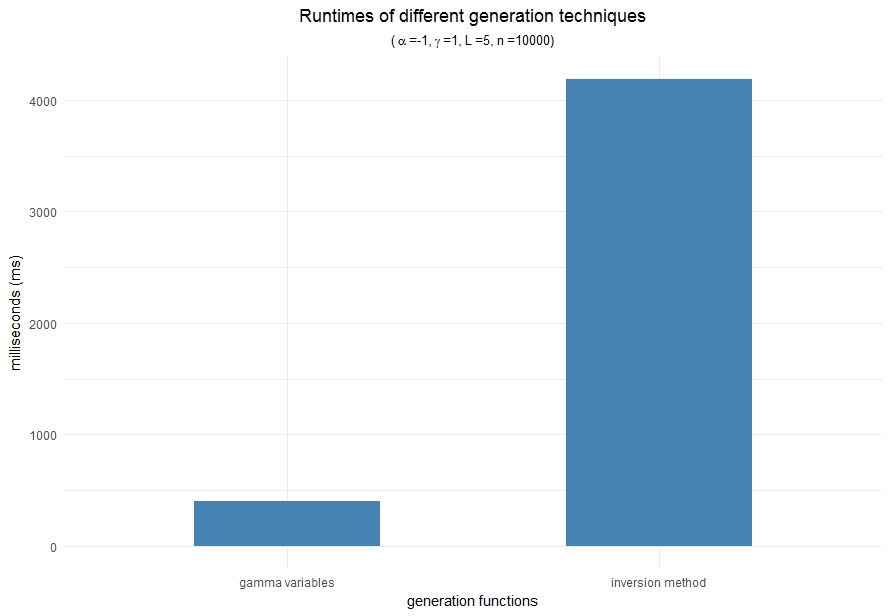
\includegraphics[width=0.95\columnwidth]{bar_L5}
	\end{center}
\end{figure}

\begin{figure}[H]
	\begin{center}
		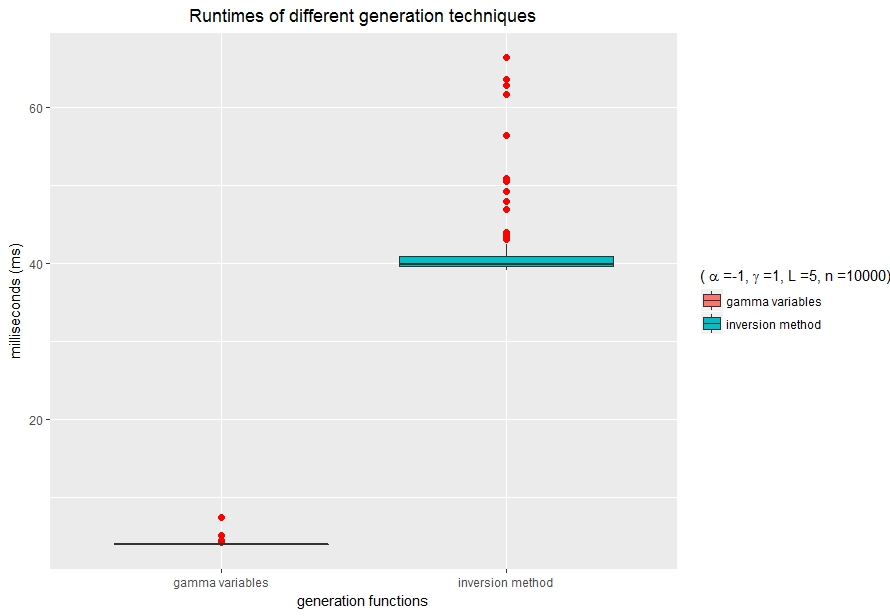
\includegraphics[width=0.95\columnwidth]{box_L5}
	\end{center}
\end{figure}

Para os parâmetros testados acima e nos demais casos testados a geração pelo Método Multiplicativo seguindo a razão das variáveis aleatórias Gamma mostrou sempre menor tempo de execução chegando a ser de 4x a 14x mais rápida em detrimento ao Método da Inversão. Assim, temos que o melhor método para se gerar as variáveis aleatórias GI0 é o método da razão de variáveis gama decorrente do Modelo Multiplicativo.

Diante desses resultados partiu-se para a parte de Estimação de parâmetros onde foram estudados diversos métodos de estimação aos quais focou-se inicialmente mais em dois: Método dos Momentos e Método da Máxima Verossimilhança. Houveram avanços teóricos de grande significância nessa parte de estimação de parâmetros, em que diversos pacotes que provém funções para calcular estimadores de parâmetros foram testados, dentre eles a biblioteca maxLik para lidar com Máxima Verossimilhança e o pacote gmm para lidar com o Método dos Momentos. Além disso, foram analisados diferentes pacotes que tratam de estimação de parâmetros para verificar se produziam resultados de estimadores confiantes e precisos.   

%=========================================================

\newpage
\section*{\centering \textbf{CONCLUSÕES}} %(máximo 2  páginas)

Portanto, em meio aos resultados decorrentes da pesquisa descritos na seção anterior, temos que os mesmos são de fato relevantes e estão de acordo com os objetivos esperados e planejados previamente pela pesquisa. Foram longos períodos de estudos dos conteúdos que estão atrelados a pesquisa para que ficasse tudo compreendido e só então após isso partia-se para a parte prática das implementações das funções.

Obtivemos resultados importantes, comparando duas técnicas bastante relevantes para geração de variáveis aleatórias em Modelos para Imagens SAR que são o Modelo Multiplicativo e o Teorema da Inversão. Por meio dos experimentos de medida de tempo verificou-se que a melhor técnica é a decorrente do Modelo Multiplicativo, evidenciando o desempenho e eficiência deste gerador.

Os fatores positivos que existiram ao longo de toda a pesquisa foi o fato de existir muitas re (livros, artigos, entre outros) referentes ao tema do projeto da pesquisa, bem como o fato de existirem seminários semanalmente no Laboratório de Computação Científica e Análise Numérica (LaCCAN) que favorecem a aquisição de novos conhecimentos a respeito de diversos temas provenientes dos demais projetos de
iniciação científica dos demais pesquisadores do laboratório. Além desses fatores positivos, podemos citar também o fato de existirem reuniões frequentes com o orientador onde puderam ser mostrados os resultados obtidos, resolvidas algumas dúvidas e traçados os novos objetivos.

	Como fatores negativos podemos citar o fato de as disciplinas da graduação
requisitarem um tempo grande o que acaba por sobrecarregar o pesquisador, além disso
houve necessidade de um tempo consideravelmente grande para estudo dos assuntos
que permeiam a área do projeto.


%=========================================================

\newpage
%REFERÊNCIAS BIBLIOGRÁFICAS (máximo 2  páginas)

\bibliographystyle{unsrt}
\bibliography{ref1}

%=========================================================

\newpage

\section*{\centering \textbf{PLANO DE TRABALHO INDIVIDUAL E DIFERENCIADO}} %(igual projeto original) 2 páginas

\textbf{Objetivos do trabalho da estudante:} Implementar uma biblioteca de
funções para a estimação de parâmetros de modelos para dados SAR e PolSAR.

\textbf{Metodologia correspondente:} Usaremos a plataforma \textit{R}. Verificaremos a qualidade numérica das funções implementadas utilizando um protocolo próprio baseado em dados simulados. Verificaremos a robustez dos algoritmos diante de possíveis problemas dos dados de entrada. Adotaremos uma versão do Modelo em Espiral de desenvolvimento de software, adaptado às necessidades do software científico.

\textbf{Cronograma de atividades:}

\textbf{Atividade 1:} Estudo das funções a serem implementadas

\textbf{Atividade 2:} Implementação e validação numérica com dados simulados

\textbf{Atividade 3:} Analise da robustez dos algoritmos com dados simulados e reais

\textbf{Atividade 4:} Construção de exemplos de uso

\textbf{Atividade 5:} Otimização do código

\textbf{Atividade 6:} Validação, verificação e preparação de manuais e tutoriais de uso

\begin{figure}[H]
	\begin{center}
		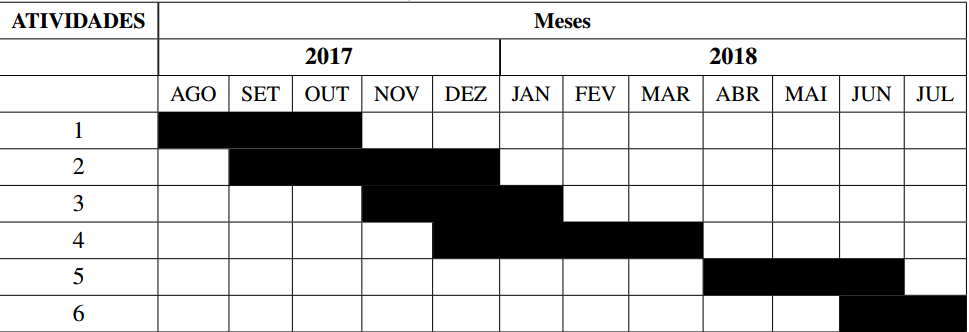
\includegraphics[width=0.95\columnwidth]{cronograma}
	\end{center}
\end{figure}

\end{document}